\chapter{Introduction}
\pagestyle{fancy}

    \section{Motivation}

        % Domain: Edge
        The rapid proliferation of real-time machine learning applications in domains such as wearable healthcare, autonomous systems, smart agriculture, and industrial automation has catalyzed a paradigm shift in embedded system design. These applications increasingly demand on-device intelligence that is not only capable of performing complex inference tasks but also optimized for low-latency responsiveness, data privacy, and long-term energy autonomy.

        % Problem of Server-based Computing
        Traditional cloud-centric architectures, where raw sensor data is transmitted to remote servers for processing, do not meet these demands. Although centralized computation offers scalability and raw performance, it introduces critical limitations for edge scenarios, most notably high communication latency, vulnerability to data breaches, and significant energy overhead due to wireless transmission. These challenges are particularly acute in applications where real-time response, user confidentiality, and prolonged battery life are essential.

        % Solution: Edge Computing
        Edge computing emerges as a compelling alternative by relocating the computation closer to the data source, either directly on the device or within its immediate environment. This architectural model addresses the fundamental constraints of modern edge deployments: minimizing latency for timely decision making, preserving privacy through local data handling, and reducing energy consumption by avoiding costly data transfers. As a result, edge computing is increasingly becoming the default execution paradigm for a new generation of smart, connected systems operating at the boundary between the physical and digital worlds.

        % Advantage 1: Reduction of Latency
        Among the most critical enablers of edge intelligence is the reduction of end-to-end latency. In cloud-based systems, sensor data must traverse potentially unreliable and congested networks before reaching remote data centers, where it is processed and subsequently returned to the device. This round-trip latency, often on the order of hundreds of milliseconds, is unacceptable for applications that demand immediate and deterministic responses.
        
        Edge computing removes this bottleneck by allowing data to be processed where it is generated. This is essential in the safety-critical and time-sensitive domains. For instance, wearable cardiac monitors must detect arrhythmias and trigger alerts in real time to avoid health risks. Similarly, precision agriculture robots must make rapid control decisions as they interact with dynamic outdoor environments. In both cases, even minor delays can degrade the reliability, efficiency, or safety of the system. Furthermore, local processing avoids the variability introduced by handovers, packet loss, or bandwidth congestion, enabling bounded and predictable response times, an essential requirement for the temporal correctness of real-time systems.

        % Advantage 2: Higher Privacy
        In addition to minimizing latency, edge computing inherently strengthens privacy by confining sensitive data to the local device. In cloud-based pipelines, information such as biomedical signals, audio recordings, or behavioral traces must traverse shared infrastructure, exposing them to risks of interception, unauthorized access, or misuse. In contrast, edge architectures reduce the attack surface by processing data locally and transmitting only aggregated or anonymized results when necessary.
        
        This localized data handling is especially critical in regulated domains such as healthcare, where compliance with privacy frameworks imposes strict restrictions on data movement, storage, and retention. Moreover, edge platforms can incorporate hardware-level security features, such as secure boot, encrypted memory, and trusted execution environments (TEEs), to ensure that privacy is not merely a software policy, but a hardware-enforced guarantee. When coupled with on-device analytics and decision-making, these protections make edge computing a robust foundation for secure and ethically sound artificial intelligence (AI) systems.

        % Advantage 3: Energy Efficiency
        Beyond latency and privacy, energy efficiency is another fundamental pillar driving the adoption of edge intelligence. Wireless communication is often one of the most power-intensive components in embedded systems, particularly when data must be continuously transmitted to remote servers. This overhead is incompatible with applications that operate under stringent energy budgets or require extended autonomous operation.
        
        By minimizing or even eliminating the need for frequent data transmission, edge computing dramatically reduces the overall energy footprint of a system. Local processing allows data to be pre-filtered, aggregated, or analyzed before any communication occurs. Furthermore, by employing task-specific accelerators and power-optimized hardware blocks, edge systems can perform computation with much lower \mbox{energy-per-operation} than general-purpose processors or cloud-based inference.
        
        This efficiency is critical in deployment scenarios such as wearable health monitors, remote sensor nodes, or implantable devices, where frequent recharging or maintenance is impractical. In such cases, energy efficiency is not just a design optimization, but a prerequisite for functional viability.

        % Sub-domain: Ultra-Low-Power Edge (TinyAI)
        As edge computing evolves, a severely constrained subdomain called ultra-low-power edge (\emph{TinyAI}) has emerged~\cite{co-design_vision}. TinyAI systems enable intelligent computation under strict power, area, and latency constraints. These platforms aim to embed AI capabilities into battery-powered devices that must function for weeks or months within power budgets of just a few tens of milliwatts, and a silicon area of only a few square millimeters.
        
        Such platforms are critical in applications where long-term autonomy, minimal invasiveness, and responsiveness must coexist. Examples include smart patches, wearable devices, and micro-scale environmental sensors. In these contexts, traditional edge design strategies must be reimagined to meet the demands of ultra-low-power, space-constrained, and real-time processing.
        
        Designing effective TinyAI systems requires careful trade-offs between performance, energy consumption, and flexibility. General-purpose central processing units (CPUs), large memory hierarchies, and conventional software stacks are often too resource-hungry. Instead, TinyAI systems must adopt lightweight processing pipelines, power-gating techniques, and deeply optimized code paths tailored to the exact workload. Ultimately, TinyAI design demands tight hardware/software co-optimization across architecture, software tooling, and application models, blurring the traditional boundaries between hardware and software development.

        % TinyAI Phases: Acquisition
        In this context, most TinyAI applications can be decomposed into two tightly coupled computational phases~\cite{bio_apps}: \emph{acquisition} and \emph{processing}. The acquisition phase involves interfacing with analog frontends to collect raw signals, such as bio-signals, environmental parameters, or audio data, through low-power analog-to-digital converters (ADCs) and peripheral interfaces~\cite{taji2024energy}. This stage requires precise control over sampling frequency, timing accuracy, and minimal power draw, especially for long-duration deployments. 

        % TinyAI Phases: Processing
        The subsequent processing phase transforms the acquired data into actionable information. This often includes digital signal processing (DSP) operations, such as filtering and feature extraction, as well as inference using lightweight machine learning models for tasks like classification or regression. These models are typically quantized and optimized for execution on minimal compute substrates, such as microcontrollers or hardware accelerators. 

        % TinyAI Phases: Overlapping
        In practice, acquisition and processing often operate in overlapping or interleaved schedules, requiring real-time synchronization, shared memory access, and fine-grained control over system timing. Efficient coordination of these phases is essential to avoid missed samples, ensure throughput, and stay within energy budgets. This coordination must be supported at both the hardware and software levels to ensure reliable and predictable behavior across application scenarios.

        % Solution: Heterogeneous Systems
        To meet these diverse and demanding constraints, \emph{heterogeneous systems} have emerged as a highly effective solution. These architectures combine a general-purpose CPU for control flow and system orchestration with one or more domain-specific accelerators~\cite{e-gpu, asip, oe-cgra, blade} that offload compute-intensive tasks, such as DSP pipelines, matrix operations, or machine learning inference.

        % Advantage 1: Flexibility 
        This architectural separation allows TinyAI systems to preserve flexibility while achieving high energy efficiency. Accelerators can be customized to match application requirements in terms of data throughput, memory access patterns, or precision, and can often be operated under strict power gating to eliminate leakage during idle periods. Meanwhile, the CPU remains responsible for managing high-level control, peripheral interfacing, and exception handling.

        % Advantage 2: Modularity
        Heterogeneous systems also support modularity and scalability. Designers can select accelerator blocks tailored to specific application domains, whether biomedical, industrial, or environmental, while leveraging a common host platform. However, this design flexibility introduces new challenges in hardware/software integration, interface standardization, and power coordination.

        % Open-Source
        Crucially, the success of such platforms depends not only on the efficiency of individual components but also on the ability to reconfigure, extend, and integrate them flexibly. These requirements make open-source hardware ecosystems, and in particular, \emph{RISC-V}, a natural foundation for the next generation of customizable TinyAI systems.
        
        The increasing complexity and specialization required by TinyAI systems have highlighted the limitations of proprietary hardware development models. Traditional system-on-chip (SoC) design often involves restrictive licensing agreements, opaque intellectual property (IP) blocks, and closed toolchains that hinder academic research, slow down innovation, and limit system-level transparency.
        
        In contrast, open-source hardware ecosystems have emerged as a disruptive force, democratizing access to high-quality IP blocks and fostering a collaborative development environment. These ecosystems enable researchers, startups, and industrial developers to customize and extend base platforms to meet specific application needs, whether by modifying microarchitectures, integrating domain-specific accelerators, or exploring new memory hierarchies.
        
        Open-source design also encourages reproducibility, peer validation, and long-term maintainability, which are essential qualities in the research-oriented and safety-critical domains. Open hardware thus provides a fertile foundation for the co-design of flexible, efficient, and extensible platforms that align with the needs of TinyAI.
        
        In particular, it allows for rapid prototyping of heterogeneous systems, seamless integration with open-source software stacks, and the ability to target multiple implementation backends, ranging from register transfer level (RTL) simulation to field programmable gate array (FPGA) emulation and application-specific integrated circuit (ASIC) tape-out.

        % RISC-V
        The success of open-source hardware in the TinyAI domain depends not only on the availability of reusable IPs but also on a well-supported, modular, and extensible instruction set architecture (ISA) to support fine-grained customization while maintaining compatibility across tools and ecosystems. This brings into focus the relevance of \emph{RISC-V}.
        
        RISC-V is a free and open ISA that has gained rapid traction in academia and industry as a foundation for processor design and system-level innovation. Unlike proprietary ISAs, RISC-V offers a modular structure: a simple base instruction set is augmented by a series of optional standard extensions (e.g., for integer multiplication, atomic operations, or floating-point arithmetic), and designers are free to implement custom extensions without breaking compatibility.
        
        This modularity makes RISC-V particularly well-suited to the development of TinyAI platforms. Designers can strip down unneeded functionality to minimize area and power or add domain-specific instructions to accelerate application-specific workloads.
        
        Moreover, the availability of a broad ecosystem of open-source RISC-V IPs, such as those of the OpenHW Group~\cite{openhw}, PULP Platform~\cite{pulp}, and other academic and commercial initiatives~\cite{opentitan}, enables plug-and-play experimentation with different trade-offs.
        
        From a system integration perspective, the RISC-V ecosystem supports open and standardized interfaces~\cite{xif}, enabling the seamless integration of custom IP blocks and accelerators into heterogeneous systems. Coupled with open-source toolchains~\cite{riscv_toolchain}, simulators~\cite{verilator}, debuggers~\cite{riscv_toolchain}, and verification frameworks~\cite{symbiyosys}, RISC-V facilitates complete end-to-end development pipelines, from RTL customization and architectural simulation to firmware and software stack development.

        % Conclusion
        To conclude, RISC-V stands out as a foundational enabler for next-generation TinyAI systems, offering an open, modular, and extensible ISA that aligns with the need for configurability, transparency, and hardware/software co-design. Its growing ecosystem of reusable IPs, standardized interfaces, and toolchains enables rapid development and integration of heterogeneous systems, supporting a range of use cases from simulation and FPGA emulation to full ASIC deployments. 

        % Gap in the state-of-the-art
        Despite the strengths of RISC-V and open-source ecosystems, there remains no cohesive, silicon-ready platform that unifies flexibility, modular accelerator integration, and accurate real-time evaluation under the severe power and area constraints of TinyAI. Existing solutions either focus on early functional prototypes without realistic performance and energy metrics or on rigid hardware designs that limit exploration of evolving workloads. This gap restricts full hardware/software co-design and slows the development of efficient, domain-specific edge intelligence.
        
        This thesis builds upon the RISC-V ecosystem to develop a cohesive set of open-source, configurable, and energy-efficient platforms for TinyAI applications. It addresses the full stack of design challenges, from real-time system prototyping and energy-accurate evaluation, to flexible microcontroller design and programmable acceleration. Through the development of reusable hardware/software infrastructures, this work aims to accelerate the research and deployment of secure, low-power, and intelligent edge devices operating under the stringent constraints of TinyAI.

    \section{Thesis Contributions}
    
        This thesis presents a comprehensive suite of technical contributions designed to address the challenges of designing and evaluating heterogeneous systems for ultra-low-power edge intelligence. The focus is on enabling flexible hardware/software co-design, efficient accelerator integration, and accurate real-time prototyping under the constraints of the TinyAI domain. These contributions span from platform-level prototyping to general-purpose programmable acceleration, all supported by open-source infrastructures. \\
        
        The main contributions of this thesis are summarized as follows:
        
        \begin{itemize}
            \item \textbf{The FEMU Framework:} The design of heterogeneous systems for TinyAI must reconcile extreme constraints in power, area, and computational resources with the need for rapid iteration and thorough evaluation. Achieving an optimal balance requires a development flow that supports functional validation, design-space exploration, and energy-aware optimization under realistic operating conditions. However, existing methodologies force a choice between accuracy and agility: RTL simulation offers detailed insight but at the cost of impractically slow execution for large workloads; high-level simulation enables faster iteration but lacks the fidelity needed for fine-grained performance and energy analysis; and FPGA-based prototyping provides a promising compromise but is often geared toward high-performance domains, requiring complex setups and offering limited support for integrated monitoring in the TinyAI context.
            
            To overcome these limitations, the first contribution of this thesis is the design of the FPGA EMUlation (FEMU)~\cite{femu}, an open-source and configurable emulation framework for prototyping and evaluating TinyAI heterogeneous systems. This approach leverages the capability of SoC-based FPGAs to combine the under-development system implemented in a reconfigurable hardware region (RH) for quick prototyping, with a software environment running under a standard operating system on a control software region (CS) for supervision and communication. The system peripherals are virtualized on the CS, while accelerators can be integrated as virtualized software models on the CS for early-stage testing or as RTL modules in the RH for later-stage development. The framework supports system-level performance and energy estimation using models derived from real-world silicon measurements. Developers interact with \mbox{FEMU} via a software interface, which simplifies communication and accelerates design space exploration.
        
            The key novelties of this work are summarized as follows:
        
            \begin{enumerate}[label=(\alph*)]
                \item \mbox{FEMU}~\cite{femu}: A reusable and modular emulation framework for prototyping and evaluating heterogeneous systems tailored for TinyAI applications.
        
                \item A hybrid hardware/software co-design strategy that enables system-level virtualization of debuggers, ADCs, and flash memories, and supports accelerator integration during both early-stage development using software models and later-stage deployment with RTL implementations.
        
                \item A system-level performance and energy estimation approach that combines runtime monitoring with technology-specific models, enabling accurate and practical system evaluation.
        
                \item \mbox{X-HEEP-FEMU}: a complete emulation platform realized by instantiating the proposed framework with real-world hardware and software components, released as open-source.

                \item A publicly released open-source repository including the complete code and documentation of \mbox{X-HEEP-FEMU} to support future research on TinyAI heterogeneous systems.\footnote{The complete code and documentation of the \mbox{X-HEEP-FEMU} platform are available at \url{https://github.com/esl-epfl/x-heep-femu} and \url{https://github.com/esl-epfl/x-heep-femu-sdk}.}
            \end{enumerate}

            Collectively, these contributions position \mbox{FEMU} as a robust and adaptable foundation for TinyAI system development, closing the gap between rapid prototyping and realistic, energy-aware evaluation. Its modular architecture, coupled with accurate performance and power modeling, empowers researchers and developers to iteratively design, integrate, and validate heterogeneous systems across the entire development cycle, from early-stage functional exploration to silicon-ready implementations.
        
            \item \textbf{The X-HEEP Platform:} While an emulation framework can accelerate the development and evaluation of TinyAI systems, its value ultimately depends on the availability of a host platform that can accommodate the diverse computational, memory, and interface requirements of heterogeneous accelerators. In practice, many open-source platforms offer only minimal configurability, focusing narrowly on the CPU core and lacking standardized mechanisms for integrating accelerators. This limited flexibility constrains the scope of architectural exploration, increases the engineering effort for each new design, and complicates the transition from prototype to silicon-ready implementations.
            
            Building on the need for flexible accelerator integration identified in the context of the \mbox{FEMU}~\cite{femu} framework, the second contribution of this thesis is the design of the eXtendible Heterogeneous Energy Efficient Platform (\mbox{X-HEEP})~\cite{x-heep}, an open-source, configurable, and extendible RISC-V platform for supporting the exploration of TinyAI accelerators. \mbox{X-HEEP} features the eXtendible Accelerator InterFace (XAIF), which enables straightforward and flexible integration of accelerators with varying interface constraints. Furthermore, \mbox{X-HEEP} provides extensive internal configurability, enabling fine-grained optimizations based on domain-specific requirements. Through its modular design, \mbox{X-HEEP} allows users to explore various hardware design trade-offs and supporting development workflows across FPGA prototyping, ASIC implementation, and mixed SystemC-RTL modeling.
        
            The key novelties of this work are summarized as follows:
        
            \begin{enumerate}[label=(\alph*)]
                \item \mbox{X-HEEP}~\cite{x-heep}: A configurable and extensible RISC-V host platform for supporting the exploration of TinyAI accelerators.
        
                \item \mbox{XAIF}: A highly adaptable accelerator interface that enables straightforward and flexible integration of accelerators with varying interface constraints.

                \item Extensive internal configurability that enables fine-grained optimizations to match application requirements.
        
                \item \mbox{HEEPocrates}~\cite{heepocrates}: A full SoC implementation in TSMC \SI{65}{\nano\meter} low-power CMOS technology, featuring the integration of a coarse-grained reconfigurable array (CGRA)~\cite{oe-cgra} and an in-memory computing (IMC)~\cite{blade} accelerator as a real-world use case of \mbox{X-HEEP}.
        
                \item A publicly released open-source repository including the complete code and documentation of \mbox{X-HEEP} to support future research on TinyAI heterogeneous systems.\footnote{The complete code and documentation of the \mbox{X-HEEP platform} are available at \url{https://github.com/esl-epfl/x-heep}.}
            \end{enumerate}

            Together, these contributions position \mbox{X-HEEP} as a versatile and silicon-ready host platform that bridges the gap between accelerator prototyping and full system deployment. By combining a modular RISC-V architecture with a highly adaptable accelerator interface and extensive internal configurability, \mbox{X-HEEP} enables seamless integration of diverse computing engines while supporting comprehensive design-space exploration across FPGA, ASIC, and mixed modeling workflows.
        
            \item \textbf{The e-GPU Platform:} Even with a flexible host platform, supporting the rapidly expanding range of TinyAI workloads requires accelerators that combine high computational efficiency with broad programmability. Domain-specific designs achieve excellent results for targeted applications but are inherently limited when algorithms evolve or new use cases emerge. Conversely, graphics processing units (GPUs) offer a versatile programming model and excel at exploiting fine-grained parallelism. Yet, existing implementations are generally too large, power-hungry, or software-heavy to operate within the strict energy, area, and runtime constraints of TinyAI devices.
            
            While most accelerators introduced in the context of the \mbox{X-HEEP} platform target domain-specific tasks, more versatile solutions are required when addressing a broader range of applications with varying demands. To address this need, the third contribution of this thesis is the design of the embedded GPU (\mbox{e-GPU})~\cite{e-gpu}, an open-source and configurable RISC-V platform for exploring the feasibility and trade-offs of utilizing GPUs in TinyAI scenarios. \mbox{e-GPU} is developed for seamless integration with \mbox{X-HEEP}~\cite{x-heep}, and its extensive configurability enables area and power optimizations to meet tight constraints. Moreover, a custom Tiny Open Computing Language (Tiny-OpenCL) implementation overcomes the compilation limitations of this domain and provides a lightweight programming framework specifically tailored for resource-constrained devices.
        
            The key novelties of this part of my PhD thesis can be summarized as follows:
        
            \begin{enumerate}[label=(\alph*)]
                \item \mbox{e-GPU}~\cite{e-gpu}, an open-source and configurable RISC-V platform for exploring the feasibility and trade-offs of using GPUs in TinyAI applications.

                \item \mbox{Tiny-OpenCL}, a lightweight OpenCL implementation tailored to resource-constrained devices to overcome the programming limitations of this application domain.
        
                \item Extensive internal configurability that enables fine-grained optimizations to match application requirements.

                \item \mbox{Accelerated processing unit (APU)}: A full system integration of e-GPU with the \mbox{X-HEEP} host to demonstrate the adaptability of the proposed platform in real-world scenarios.
        
                \item A publicly released open-source repository including the complete code and documentation of \mbox{e-GPU} to support future research on TinyAI heterogeneous systems.\footnote{The complete code and documentation of the e-GPU platform are available at \url{https://github.com/esl-epfl/e-gpu}.}
            \end{enumerate}

            These contributions position \mbox{e-GPU} as a compact and adaptable GPU-based accelerator capable of delivering high parallel performance within the stringent power and area constraints of TinyAI systems. Its tight integration with \mbox{X-HEEP}, combined with extensive configurability and a lightweight programming framework, enables efficient execution of a wide range of workloads while preserving the flexibility needed to adapt to evolving application demands.
        
        \end{itemize}
        
        All novelties in this thesis follow a vertically integrated hardware/software co-design methodology. Hosts, accelerators, memory systems, and toolchains are jointly optimized to meet the performance, area, and energy requirements of TinyAI applications. Furthermore, all platforms and tools developed in this work, \mbox{X-HEEP-FEMU}, \mbox{X-HEEP}, and \mbox{e-GPU} are released under permissive open-source licenses. This ensures reproducibility, transparency, and extensibility, and provides the research community with a modular and interoperable infrastructure to explore configurable and efficient heterogeneous systems for the next generation of TinyAI devices.

    \section{Thesis Use Case}
    
        Beyond their individual roles, the three proposed platforms --- \mbox{X-HEEP-FEMU}, \mbox{X-HEEP}, and \mbox{e-GPU} --- collectively constitute a unified and complementary framework that supports the entire life cycle of TinyAI system design, from initial functional prototyping to quantitative architectural evaluation. Their combined adoption enables researchers and designers to efficiently explore, implement, and benchmark heterogeneous systems tailored to the stringent power, area, and performance constraints of ultra-low-power applications.
        
        \begin{itemize}
            \item \textbf{Accelerator exploration and early prototyping:} The design process typically begins with the exploration of a new accelerator concept targeting a representative TinyAI workload, such as biomedical signal analysis, event-based sensing, or environmental monitoring. In this early phase, the \mbox{X-HEEP-FEMU} platform provides an instrumented and virtualized environment in which the accelerator model can be integrated, validated, and evaluated before hardware implementation. Using its hardware virtualization capabilities, designers can test accelerator software models under realistic timing and communication conditions. This approach greatly reduces the turnaround time between algorithmic exploration and hardware realization, promoting rapid and iterative refinement of the design.
        
            \item \textbf{Integration and system-level evaluation:} Once the accelerator reaches functional maturity, it can be seamlessly integrated within the \mbox{X-HEEP} host platform. Through the XAIF interface, \mbox{X-HEEP} provides standardized communication, synchronization, and memory-access mechanisms, enabling the connection of accelerators with diverse bandwidth, latency, and power characteristics. This stage allows designers to refine the accelerator architecture and evaluate hardware interactions under realistic TinyAI operating conditions. During this phase, the \mbox{X-HEEP-FEMU} infrastructure is employed to estimate performance and energy, providing accurate and reproducible metrics to guide design-space exploration and architectural optimization. Moreover, the multi-target nature of \mbox{X-HEEP}, which supports both FPGA and ASIC back-ends, facilitates the transition from emulated prototypes to silicon-ready implementations, ensuring architectural consistency and reusability across all design stages.
        
            \item \textbf{Comparative analysis and benchmarking:} To assess the effectiveness of the proposed accelerator within the TinyAI domain, its performance and energy efficiency can be quantitatively compared against multiple reference architectures. These include the RISC-V CPU subsystem integrated in \mbox{X-HEEP}, representing the general-purpose computing baseline, and the programmable \mbox{e-GPU} accelerator, which serves as a data-parallel reference architecture. Workloads executed on the \mbox{e-GPU} leverage the lightweight \emph{Tiny-OpenCL} runtime, enabling portable kernel compilation and efficient mapping to its parallel execution model. This comparative approach provides a systematic means to quantify the benefits and limitations of the accelerator under design with respect to general-purpose and programmable parallel architectures, offering a comprehensive assessment of its performance, programmability, and energy efficiency within heterogeneous TinyAI systems.
        \end{itemize}
        
        Collectively, these three platforms define a coherent and reproducible methodology that bridges functional prototyping, hardware integration, and architectural benchmarking within a single open-source ecosystem. This unified flow enables researchers to progress seamlessly from high-level accelerator concepts to fully realized heterogeneous systems validated in hardware and characterized under realistic workloads.
        
    \section{Thesis Outline}
        
        This thesis is organized into five chapters, each building upon the previous to address a different challenge to enable efficient, low-power, and programmable TinyAI heterogeneous systems through open-source and configurable RISC-V-based platforms. The structure reflects a natural progression, from the need for real-time prototyping to accelerator integration and programmable data-parallel computing.
        
        \noindent\textbf{Chapter~2} introduces \emph{FEMU}~\cite{femu}, an SoC-based FPGA framework designed to prototype and evaluate TinyAI systems under realistic conditions. This chapter presents the motivation for FEMU in response to the limitations of both RTL simulation and software-based approaches, highlighting the need for real-time execution, flexible IP virtualization, and reliable performance and energy estimations. A complete instantiation of the framework, called \mbox{X-HEEP-FEMU}, is presented as a reference platform and evaluated using representative acquisition and processing workloads.
        
        \noindent\textbf{Chapter~3} builds on this foundation by presenting \emph{X-HEEP}~\cite{x-heep}, a flexible and modular RISC-V host platform that flexibly integrates within \mbox{FEMU} for supporting the exploration of accelerators. The chapter introduces the configurability and extendability features of \mbox{X-HEEP}, which enable the seamless integration of accelerators with varying bandwidth, latency, and programmability requirements. As a case study, the chapter presents \mbox{HEEPocrates}, an ASIC implementation fabricated in TSMC \SI{65}{\nano\meter} low-power CMOS technology, and evaluates it against reference platforms.
        
        \noindent\textbf{Chapter~4} shifts focus from domain-specific to general-purpose acceleration by introducing \emph{e-GPU}~\cite{e-gpu}, a lightweight and configurable RISC-V GPU tailored for the TinyAI domain. While prior chapters focus on fixed-function accelerators, this chapter explores the feasibility and trade-offs of general-purpose data-parallel execution under strict power and area constraints. It presents the architecture of e-GPU, its configuration knobs, and the \mbox{Tiny-OpenCL} runtime environment developed for constrained devices. A complete APU, which integrates \mbox{e-GPU} with \mbox{X-HEEP}, is presented as a use case and evaluated with representative workloads.
        
        \noindent\textbf{Chapter~5} concludes the thesis by summarizing the main contributions in all chapters and reflecting on their collective impact on TinyAI hardware/software co-design. It also discusses future research directions, highlighting potential extensions of the proposed platforms to support increasingly complex workloads, tighter power budgets, and broader integration within emerging TinyAI ecosystems.

        \begin{figure} [t]
            \centering
            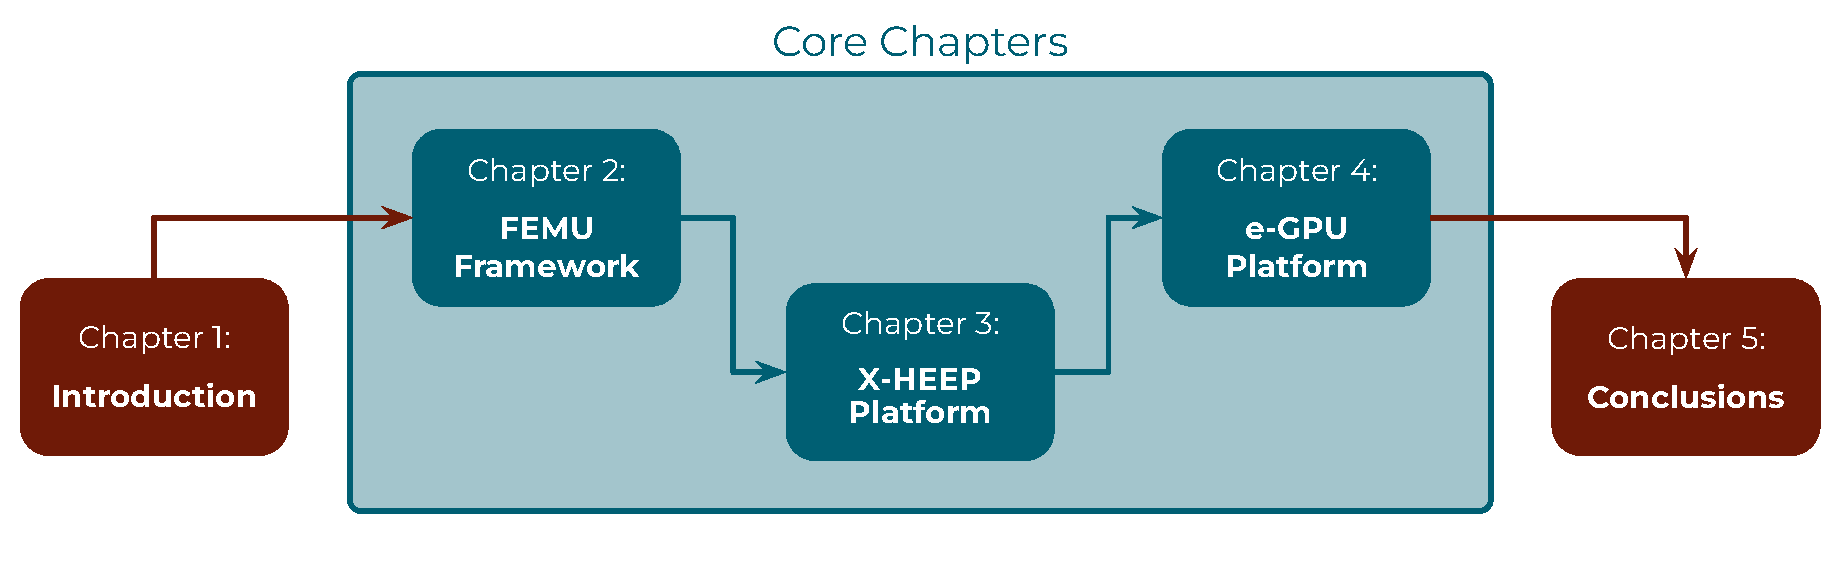
\includegraphics[width=1\textwidth]{./figures_intro/thesis_flow.pdf}
            \caption{Block diagram of the thesis structure and contribution flow.}
            \label{fig:thesis_flow}
        \end{figure}
